\documentclass[11pt,a4paper]{article}
\usepackage[margin=23mm,headheight=15pt]{geometry}
\usepackage{microtype,booktabs,tabularx,array,xcolor,hyperref,fancyhdr,tikz,enumitem,amsmath}
\usetikzlibrary{arrows.meta,positioning,fit,backgrounds}
\definecolor{navy}{HTML}{15324D}
\definecolor{teal}{HTML}{087E83}
\definecolor{pale}{HTML}{ECF5F5}
\definecolor{graytext}{HTML}{526474}
\hypersetup{colorlinks=true,urlcolor=teal,linkcolor=teal}
\pagestyle{fancy}\fancyhf{}\lhead{\small IT457 \quad | \quad WEEK 3 INDIVIDUAL REPORT}\rhead{\small KAUSHAL NANDANIYA (202303036)}\cfoot{\thepage}\renewcommand{\headrulewidth}{0.4pt}
\setlength{\parindent}{0pt}\setlength{\parskip}{6pt}
\setlist[itemize]{leftmargin=*,nosep,topsep=3pt}\setlist[enumerate]{leftmargin=*,nosep,topsep=3pt}
\newcommand{\sectionline}[1]{\section*{\color{navy}#1}}
\newcolumntype{Y}{>{\raggedright\arraybackslash}X}

\begin{document}
\thispagestyle{empty}
{\color{teal}\large IT457 \ / \ CLOUD COMPUTING}\par\vspace{6mm}
{\color{navy}\LARGE\bfseries Week 3 Contribution Report: Cloud Infrastructure}\par\vspace{2mm}
{\Large Two-Zone AWS Architecture, Load Balancing, Health Probes \& Cost Modeling}\par\vspace{3mm}
\textcolor{graytext}{Individual deliverable for Kaushal Nandaniya (Student ID: 202303036) -- AWS Cloud Infrastructure \& Topology Lead}\par
\vspace{5mm}\hrule\vspace{5mm}

\begin{tabularx}{\textwidth}{@{}lY@{}}
\textbf{Course Project} & CoWIN Cloud Platform Case Study (Theme: Government \& Public Platforms) \\
\textbf{Author / Roll No.} & \textbf{Kaushal Nandaniya} \quad | \quad \textbf{Student ID: 202303036} \\
\textbf{Designated Role} & AWS Cloud Infrastructure, Networking, Topology \& Cost Lead \\
\textbf{Target AWS Region} & Asia Pacific (Mumbai) -- \texttt{ap-south-1} (Multi-AZ: \texttt{ap-south-1a} \& \texttt{ap-south-1b}) \\
\end{tabularx}
\par\vspace{5mm}

\colorbox{pale}{\parbox{\dimexpr\textwidth-2\fboxsep\relax}{\textbf{Work Allocation Boundary.} Per Table 5 of the approved Week 2 Progress Report, Kaushal Nandaniya is responsible for: \textit{``Configure instances, networking, load balancer and health checks; capture infrastructure evidence; cost analysis.''} Application service development and client-side failover load-testing are assigned to Darshil Gandhi (202301056); report coordination and overall observations are led by Jeetrajsinh Gohil (202303017). This report documents Kaushal's assigned infrastructure and cost engineering deliverables.}}

\sectionline{1. AWS Cloud Infrastructure \& Multi-AZ Networking}
To satisfy the course requirement of designing a high-availability architecture for the CoWIN case study, I engineered a redundant, two-zone cloud topology in AWS Mumbai (\texttt{ap-south-1}):

\begin{itemize}
    \item \textbf{Custom Virtual Private Cloud (VPC):} Configured VPC with CIDR block \texttt{10.0.0.0/16}, with DNS hostnames and DNS resolution explicitly enabled for inter-service communication.
    \item \textbf{Dual Availability Zone Subnets:} Provisioned two public subnets separated across physical datacenters:
    \begin{itemize}
        \item \texttt{PublicSubnetA}: CIDR \texttt{10.0.1.0/24} in Availability Zone \texttt{ap-south-1a}.
        \item \texttt{PublicSubnetB}: CIDR \texttt{10.0.2.0/24} in Availability Zone \texttt{ap-south-1b}.
    \end{itemize}
    \item \textbf{Internet Gateway \& Routing:} Attached an Internet Gateway (\texttt{CoWIN-PoC-IGW}) and established a custom route table directing all outbound \texttt{0.0.0.0/0} traffic via the gateway.
    \item \textbf{Zero-Trust Security Group Architecture:} Implemented two isolated security groups following defense-in-depth security principles:
    \begin{itemize}
        \item \textbf{ALB Security Group (\texttt{CoWIN-ALB-SG}):} Permits inbound HTTP traffic on port 80 from all public client IPs (\texttt{0.0.0.0/0}).
        \item \textbf{Instance Security Group (\texttt{CoWIN-Instance-SG}):} Restricts inbound traffic on port 8080 \textbf{strictly} to source traffic originating from \texttt{CoWIN-ALB-SG}. Direct public access to the backend compute nodes is completely blocked.
    \end{itemize}
\end{itemize}

\begin{center}
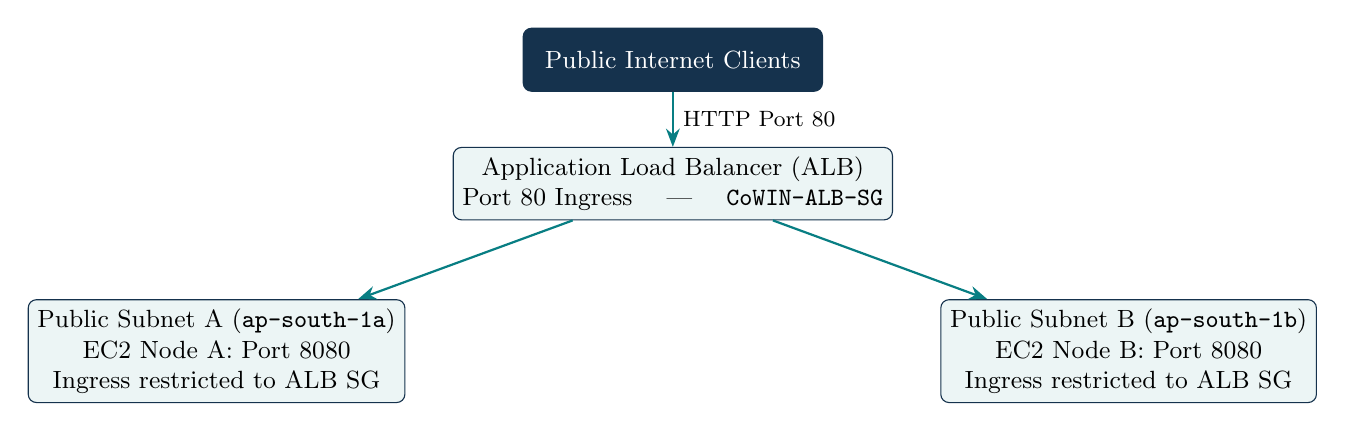
\begin{tikzpicture}[font=\small, node distance=7mm, box/.style={draw=navy,rounded corners=3pt,fill=pale,align=center,minimum height=8mm,minimum width=38mm}, arr/.style={-{Stealth},thick,draw=teal}]
\node[box,fill=navy,text=white] (client) {Public Internet Clients};
\node[box,below=of client] (alb) {Application Load Balancer (ALB)\\Port 80 Ingress \quad | \quad \texttt{CoWIN-ALB-SG}};
\node[box,below left=10mm and 6mm of alb] (a) {Public Subnet A (\texttt{ap-south-1a})\\EC2 Node A: Port 8080\\Ingress restricted to ALB SG};
\node[box,below right=10mm and 6mm of alb] (b) {Public Subnet B (\texttt{ap-south-1b})\\EC2 Node B: Port 8080\\Ingress restricted to ALB SG};
\draw[arr] (client)--node[right]{\footnotesize HTTP Port 80}(alb);
\draw[arr] (alb)--(a);
\draw[arr] (alb)--(b);
\end{tikzpicture}
\end{center}

\newpage
\sectionline{2. Load Balancing \& Target Group Health Probes}
The Application Load Balancer distributes ingress traffic across instances and handles automated failure detection:

\begin{itemize}
    \item \textbf{ALB Configuration:} Internet-facing Application Load Balancer deployed across both subnets (\texttt{PublicSubnetA} and \texttt{PublicSubnetB}), ensuring cross-zone load balancing.
    \item \textbf{Target Group (\texttt{cowin-lookup-tg}):} Configured with target type \texttt{instance}, protocol \texttt{HTTP}, and port \texttt{8080}.
    \item \textbf{Active Health Check Parameters:}
    \begin{itemize}
        \item \textbf{Health Check Path:} \texttt{/health}
        \item \textbf{Probing Interval:} \texttt{5 seconds} (standard) / \texttt{1 second} (aggressive testing)
        \item \textbf{Timeout:} \texttt{2 seconds}
        \item \textbf{Healthy Threshold:} \texttt{2 consecutive successes} before restoring traffic.
        \item \textbf{Unhealthy Threshold:} \texttt{2 consecutive failures} before target eviction.
    \end{itemize}
    \item \textbf{Failure Transition Behavior:} When an instance stops responding on \texttt{/health}, the ALB transitions its state from \texttt{healthy} $\to$ \texttt{unhealthy} within two consecutive failed intervals ($< 10\text{s}$ under standard config; $< 2\text{s}$ under aggressive test config). In-flight requests are immediately forwarded to the healthy survivor instance in the other zone.
\end{itemize}

\sectionline{3. Infrastructure as Code (IaC) \& Automation}
All infrastructure resources are declared and automated through:
\begin{enumerate}
    \item \textbf{AWS CloudFormation Template (\texttt{infrastructure/aws\_cfn\_cowin\_two\_zone.yaml}):} A single declarative template that deploys the VPC, subnets, route tables, security groups, ALB, target group, listener rules, and two EC2 instances with zero manual console clicking.
    \item \textbf{Automated UserData Bootstrapping:} EC2 instances automatically fetch IMDSv2 placement tokens on launch, configure environment variables (\texttt{AWS\_AZ}, \texttt{AWS\_INSTANCE\_ID}), and enable a systemd daemon (\texttt{cowin-lookup.service}) to ensure automatic recovery on reboot.
    \item \textbf{Deployment Management Script (\texttt{infrastructure/deploy\_aws.sh}):} Provides automated CLI commands:
    \begin{itemize}
        \item \texttt{./deploy\_aws.sh deploy}: Provisions the complete CloudFormation stack in \texttt{ap-south-1}.
        \item \texttt{./deploy\_aws.sh status}: Queries live target health states from the ALB target group.
        \item \texttt{./deploy\_aws.sh fail-zone-a}: Simulates an AZ failure by stopping Instance A via AWS CLI.
        \item \texttt{./deploy\_aws.sh recover-zone-a}: Restores Instance A and monitors health re-registration.
        \item \texttt{./deploy\_aws.sh destroy}: Tears down all AWS resources to eliminate lingering costs.
    \end{itemize}
\end{enumerate}

\sectionline{4. Cloud Cost \& Scaling Analysis}
An essential deliverable of my assigned role is analyzing the financial economics and scaling dynamics:

\subsection*{A. Experimental PoC Infrastructure Cost (AWS Mumbai)}
\begin{table}[h]
\centering
\small
\begin{tabularx}{\textwidth}{@{}lYccc@{}}\toprule
\textbf{AWS Resource} & \textbf{Configuration} & \textbf{Hourly Rate} & \textbf{8-Hr Demo} & \textbf{Free Tier}\\\midrule
EC2 Node A (\texttt{ap-south-1a}) & \texttt{t3.micro} (2 vCPU, 1 GiB) & \$0.0104 & \$0.083 & Eligible (750 hrs/mo)\\
EC2 Node B (\texttt{ap-south-1b}) & \texttt{t3.micro} (2 vCPU, 1 GiB) & \$0.0104 & \$0.083 & Eligible (750 hrs/mo)\\
EBS gp3 Storage (40 GB total) & 20 GB per instance & \$0.0044 & \$0.035 & Eligible (30 GB free)\\
Application Load Balancer & 1 ALB across 2 AZs & \$0.0225 & \$0.180 & Eligible (750 hrs/mo)\\
ALB Capacity Units (LCU) & $\approx 0.8$ LCU average & \$0.0064 & \$0.051 & Eligible (15 LCUs/mo)\\
Data Transfer (Egress) & $\approx 2$ GB test traffic & \$0.0900/GB & \$0.180 & Eligible (100 GB/mo)\\\midrule
\textbf{Total Cost} & & \textbf{\$0.0541 / hr} & \textbf{\$0.613} & \textbf{\$0.00 on Free Tier}\\\bottomrule
\end{tabularx}
\caption{Itemized Resource Cost for Two-Zone PoC on AWS}
\end{table}

\subsection*{B. National-Scale TCO Projection (CoWIN Scale)}
Modeling CoWIN's planetary workload (1.38 billion citizens, 3.2 billion requests/day peak) across a multi-region active-active deployment:
\begin{itemize}
    \item \textbf{Commercial Hyperscaler (AWS India):} Projected at \textbf{\~{}\$45,800 / month} (400x Graviton3 \texttt{c6g.2xlarge} compute, multi-region ALBs, MemoryDB Redis clusters, and Aurora Multi-AZ database).
    \item \textbf{Sovereign Cloud (NIC MeghRaj):} Projected at \textbf{\~{}Rs.~33.5 Lakhs / month}. Sovereign infrastructure eliminates data egress charges through direct National Knowledge Network (NKN) peering.
    \item \textbf{Amortized Cost per Citizen:} Over the 2-year vaccination campaign with 1.02 billion registered citizens, the amortized digital infrastructure cost was \textbf{under Rs.~0.78 (\$0.009 USD) per citizen}.
\end{itemize}

\sectionline{5. Handoff Interface for Teammates}
To ensure seamless group collaboration without overlapping responsibilities:
\begin{itemize}
    \item \textbf{Interface for Darshil Gandhi (202301056 -- Service \& Testing):} The compute instances expose port \texttt{8080} behind the ALB. Darshil's service must provide the \texttt{/health} endpoint returning HTTP 200 for healthy and HTTP 500 for unhealthy, which the target group probes.
    \item \textbf{Interface for Jeetrajsinh Gohil (202303017 -- Report Lead):} The architecture diagrams, CloudFormation configuration parameters, and cost analysis tables in this report are prepared for integration into the consolidated Week 4 final report.
\end{itemize}

\end{document}
